\section{Applications}
\label{ch:app}

\epigraph{Simplicity is Complicated.}{Rob Pike}

This chapter we first introduce a possible application of our proposed model
including the implemented feature, how it could benefit a user, as well as the 
architecture and dataflow within the application.
Then in the second part of this chapter, we formalize and discusse 
the possibility and benefits as a standard Web API to web developers and website designer.

\subsection{Client-side Browser Plugin}
\label{sec:plugin}

We developed a client-side browser plugin is an illustration of our model applications.
The plugin is an intelligent system that proactively serves its user, 
and it provides proactive notification based on the historical actions in a session
when browsing behavior is detected as goal-oriented or fuzzy behavior, 
as illustrated in Figure \ref{fig:proactive-noti}.

\begin{figure}[H]
    \centering
    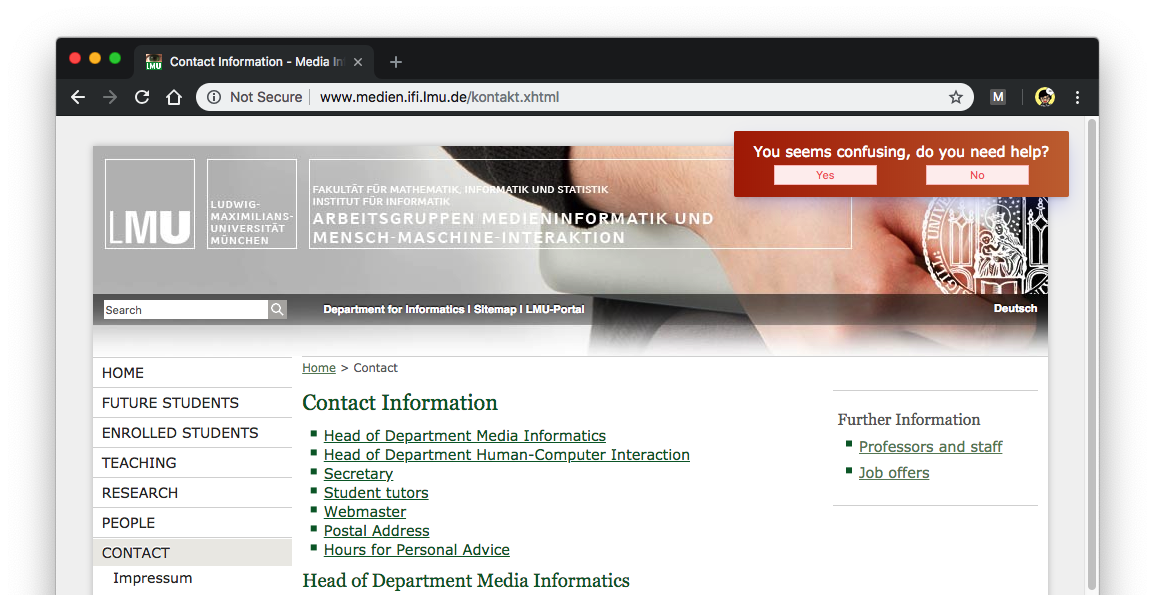
\includegraphics[width=0.7\textwidth]{figures/proactive-noti}
    \caption{Proactive notification:
    The plugin injects monitor script when the page is loaded, and then serve user giving
    notification when detecting fuzzy browsing behavior.}
    \label{fig:proactive-noti}
\end{figure}

The user can either select ``Yes'' and navigates to the most likely page that he/she will visit
in the future, or select ``No'' to ignore the notification.
The plugin serves user only if the browsing behavior is detected as fuzzy behavior because
of the forbear of notification. We argue that the plugin is only a supplementary of improving
browsing experience but not always necessary, for instance in exploring behavior, information
need of a user may not be clearly observed and the recommendations are not usefulness. 
One of the benefits of the plugin is to proactively help the user become efficient
and reach the destination as fast as possible in goal-oriented browsing.

\begin{figure}[H]
    \centering
    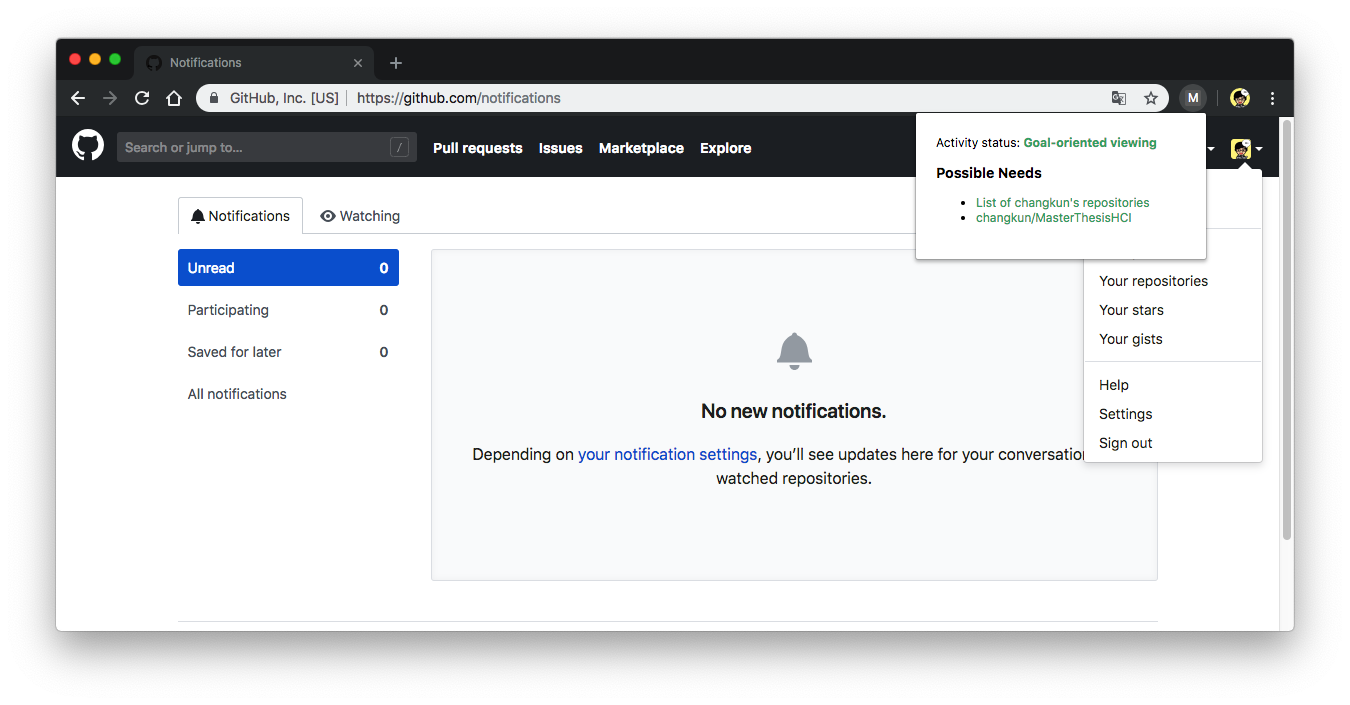
\includegraphics[width=0.7\textwidth]{figures/plugin-predicting-result}
    \caption{The plugin provided popup page: users can always open the page
    to understand the current status of browsing and predicted needs based on
    historical actions in a browsing session. In this case, the detected browsing behavior
    is under goal-oriented browsing, and predicted actions
    are accessing the page of public repositories and accessing a specific repository.}
    \label{fig:plugin-predict}
\end{figure}

In Figure \ref{fig:plugin-predict}, except proactive notification, 
users can always open a popup page provided by the plugin.
The popup page provides another interaction that gives the predicted needs 
based on historical user actions. A user can always interact with the plugin and
retrieve the possible needs and browsing status in the current session.
These information are helpful to the plugin user because the user can understand
what is the current status of web browsing, which implicitly aware the person better focus
if the person detected as exploring browsing behavior.

\begin{figure}[H]
    \centering
    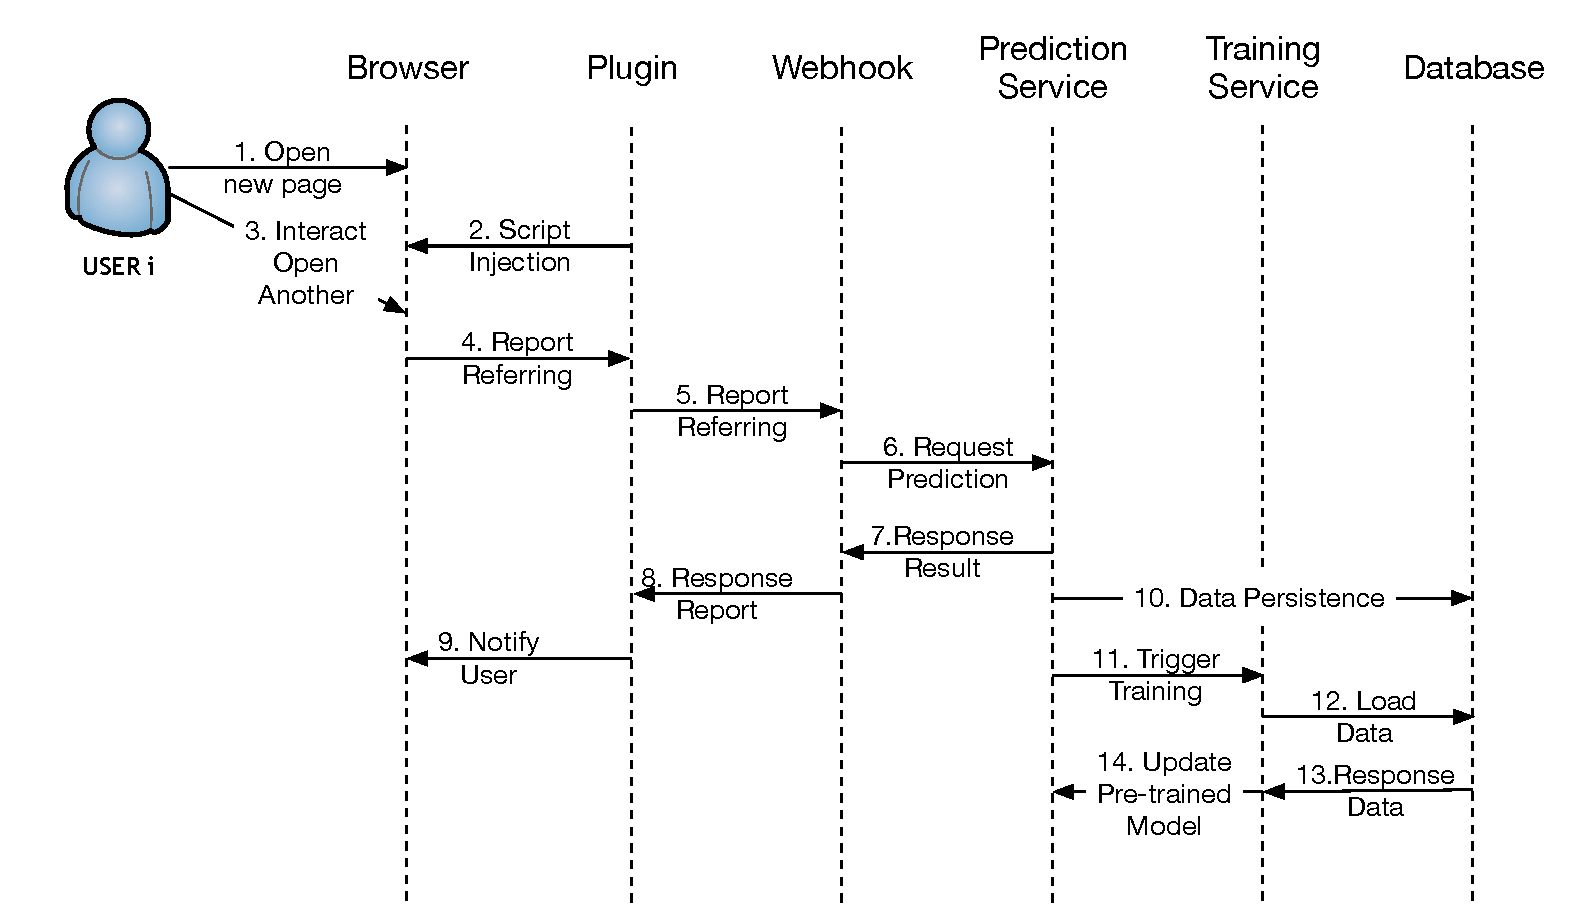
\includegraphics[width=0.7\textwidth]{figures/arch}
    \caption{The implemented architecture of our plugin}
    \label{fig:arch}
\end{figure}

The implementation and architecture is not simple
despite it provides a small feature that exhibit context and future inforamtion to the user.
Figure \ref{fig:arch} illustrates the implemented architecture of the plugin.

First of all, the plugin daemon process will inject monitoring script (\emph{step2}) to 
the newly opened page (\emph{step1}).
When user start browsing and interacting (\emph{step3}), the injected script will report the referring of
previous visited URL, current URL and stay duration to the daemon process of the plugin (\emph{step4}).

Afterwards, the daemon process will report the referring information to the plguin server webhook (\emph{step5}),
and then the webhook will immediatelly request the intra prediction microservice (\emph{step6}) and resulting a 
prediction (\emph{step7}) then response a prediction result to the daemon process 
by using a pre-trained model (\emph{step8}). Therefore the daemon process can decide 
if a proactive notification should be presented to the user or simply update its popup page
just for illustration (\emph{step9}).

Since the prediction service received a new user action, it stores the action into database
subsequently for model update (\emph{step10}). Because of the cost of train a new model,
the prediction service can decide to trigger training service to retrain the model 
if already received enough new data (\emph{step11}). 
Further, the training service uses the pre-trained model as
a base model to initiate the training by request newly created data from databse (\emph{step12} and \emph{step13}), 
similar to the idea of transfer learning.
After the training achieved a compatible performance comparing to the pre-trained model,
the training service will update the newly trained model to the prediction service (\emph{step14}), which 
serves future prediciton requests.

As we can observe from the architecture, the infrastructure is not as simple as the plugin feature
intent to provide, therefore we argue that it is a feature that only browser manufactures
can provide. In the following section, we formalize and discuss 
the possibilities of the plugin feature as a Web API.

\subsection{Web API Standardization and Platform-as-a-Service}

Web APIs is a generic term used in various fields of development.
Web APIs in a context of web browsers mainly indicates the APIs provided
by browser manufactures to developers that helps web application can even close
to manipulate hardwares, for instance, WebAssembly \cite{w3c2018ws}.

Nowadays, there are experimental standard Web APIs integrates complex features to 
web developers, e.g. Web Speech APIs \cite{mozilla2019speech}, and 
only Google Chrome (after version 24) support. 
The specification proposal was initiated by Google, according to 
the source code of Chromium Kernel, the APIs are implemented based on 
the speech recognition service provided 
by Google Cloud Platform 
\footnote{\url{https://github.com/chromium/chromium/blob/83928864c18362a4b0f84bad9bee4104f4655430/content/browser/speech/speech\_recognition\_engine.cc\#L35}, last accessed on January 03, 2019},
which provides us a signal that browser APIs does not only giving interfaces to
the hardware, but also access cloud platform services, i.e. Platform-as-a-Service integrated 
APIs.

The plugin we illustrated in Section \ref{sec:plugin} can also be integrated as a PaaS API
that embedded into web browsers, which simplifies the infrastructure of the plugin. 
As a developer, one can simply call the standardized API to report current user actions
then get a response of current behavior status and the prediction of future movement or 
actions, as the diagram shown in Figure \ref{fig:webapi}.

\begin{figure}[H]
    \centering
    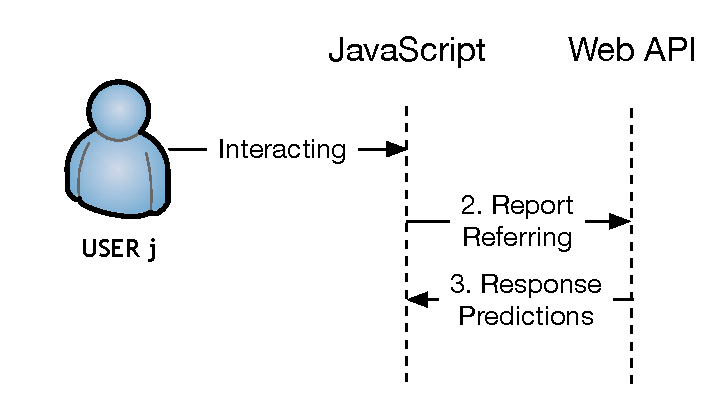
\includegraphics[width=0.4\textwidth]{figures/webapi}
    \caption{Usage overview of standadized BrowsingBehavior API}
    \label{fig:webapi}
\end{figure}

Defining the specification of the Paas API aims enable web developers to
monitoring, in a web browser, the future actions of their user.
Developers can use the predicted actions to dynamically change the UI elements then improve
the user experience of their product. To keep the API to a minimum, we breifly discuss the
non-normative web API design of the browsing behavior predictor.

\subsubsection{The \emph{BrowsingBehavior} Interface}

The browsing behavior interface is the scripted web API for resulting a monitored browsing
session, which is presented in Code \ref{lst:interface}.

\begin{lstlisting}[
    language={JavaScript},
    caption={BrowsingBehavior Interface},
    label={lst:interface}
]
[Exposed=Window, Constructor]
interface BrowsingBehavior : EventTarget {
    
    // methods to drive browsing behavior response
    void start();
    void stop();
    void pause();
    void resume();

    // event methods
    attribute EventHandler onBrowsingStart;
    attribute EventHandler onBrowsingEnd;
    attribute EventHandler onBrowsingPause;
    attribute EventHandler onBrowsingResume;
    attribute EventHandler onResult;
}
\end{lstlisting}

\paragraph{\emph{start()} method} When start method is called, it represents the moment in
time the web application wishes to begin monitoring user's actions.
Then every step when user making actions, the \emph{EventHandler onResult} will produce
a standard prediction and classification of user browsing behavior. Further, 
the \emph{EventHandler onBrowsingStart} will be called immediatelly after calling 
this method and before resulting a prediction result, which gives a barrier in between of
calling \emph{start} and callback \emph{onResult}.

\paragraph{\emph{stop()} method} When stop method is called, it represents the instruction
to browsing behavior service to stop monitoring user actions, and resulting a final 
prediction in the \emph{EventHandler onBrowsingEnd}.

\paragraph{\emph{pause()} method} This method is used to ignoring the upcoming user actions
to pauses the monitoring of user actions, and resulting a prediction in the 
\emph{EventHandler onBrowsingPause}.

\paragraph{\emph{resume()} method} This method resumes the paused \emph{BrowsingBehavior}
object and recover the monitoring of user actions. Before monitoring is fully recovered,
the \emph{EventHandler onBrowsingResume} will be called.

The major consideration of designing these four methods is to restrict an abuse of the APIs.
Similar to cookie, speech recognition APIs, a website should acquire an authorization from
their user, otherwise the API cannot monitor any user actions on the web, which partially
solves the issue of privacy and security. We will discuss more concerns of the feature in
Chapter \ref{ch:discuss}.

\subsubsection{\emph{onResult} callback}

\emph{onResult} callback passes the prediction after the browser user performed an action.
The prediction result consist two parts: behavior and future movements.

The \emph{behavior} attribute of the result object is a JSON object that contains 
confidence level, i.e. classification probability, and a enumerate \emph{category} attribute
that indicate the a finite set of user browsing behaviors, i.e. goal-oriented, fuzzy or exploring.

\begin{lstlisting}[
    language={JavaScript},
    caption={Result object of onResult callback},
    label={lst:callback}
]
{
    "behavior": {
        "confidence": float64,
        "category": string,
    },
    "futures": [
        {
            "confidence": float64,
            "actions": array[string],
        },
        {
            "confidence": float64,
            "actions": array[string],
        },
        ...
    ]
}
\end{lstlisting}

The \emph{futures} attribute of the result object is an ordered JSON object that from the
highest \emph{confidence} to lowerest {confidence} and the \emph{confidence} is a floating
number from minimum 0 to maximum 1 value. Meanwhile, the \emph{actions} attribute in a 
JSON object of an item of \emph{futures} array is an array of possible actions of URLs that
ordered in chronologic order, the first element represents the next immediate action,
and the last element represents the final action in the session, as shown in Code \ref{lst:callback}.

\begin{lstlisting}[
    language={JavaScript},
    caption={Formation of browser collections},
    label={lst:collect}
]
{
    "device_id": string,
    "previous_url": string,
    "current_url": string,
    "stay_seconds": float64,
    "time": string
}
\end{lstlisting}

From the perspective of implementation, browser manufactures collect data after developer
calls \emph{start()}.
In Code \ref{lst:collect}, each time when user performs an action, including open a new page,
switch to another tab or backtrack to former page, will result an JSON object that contains
\emph{device\_id} a unique identifier that represents the device, \emph{previous\_url} the previous
URL of the action, \emph{current\_url} the current URL of the action, \emph{stay\_seconds}
the stay duration of \emph{previous\_url} and \emph{time} string of the time of data creation.

% \subsubsection{Communication Protocol}

\cleardoublepage